% !TeX root = ../../thesis.tex
\chapter{Applications: Acetabular cup}\label{ch:cup}

\begin{shaded}
This chapter is based on prepared manuscript to be submitted to  \textit{IEEE Computing in Science \& Engineering}:\\
M. Barzegari, F. Perez-Boerema, G. Zavodszky, and L. Geris, ``High-performance computer simulation of biodegradation of optimized personalized implants; a case study of a patient-specific porous acetabular implant,'' will be submitted to \textit{IEEE Computing in Science \& Engineering}.
\end{shaded}

\section{Introduction}


%From a biodegradation perspective, biomaterials can be classified into two categories: bio-inert and biodegradable. Although bio-inert biomaterials show a great performance especially in fixation applications, they bring an important problem into the play: they remain in the body forever or require additional surgery to remove them. Biodegradable materials do not have this problem, and in case of metallic biomaterials, they also provide a dynamic (i.e. time-varying) mechanical stability profile, but taking advantage of them requires tuning the degradation parameters and material release rate.

%Developing a quantitative mathematical model of the degradation process is a proper solution to this issue by allowing researchers to study the biodegradation behavior of any desired implant in-silico (in the computer) prior to conducting any in-vitro or in-vivo experiments. Developed mathematical models can be simulated using efficient numerical schemes such as the finite element method. The primary challenge here will be achieving a high accuracy at the interface between the implant and surrounding tissue in the body as the interface plays an important role in the degradation phenomena. Increased accuracy means increased computational cost and resources (especially time), but high-performance computing (HPC) techniques can be used to overcome this challenge.

Before we can take advantage of the interesting properties of metallic biodegradable implants, their biodegradation behavior needs to be evaluated and tuned for the target application. One example from orthopedics is tuning the degradation rate of implants to match the rate of bone formation. \textit{In silico} models can be beneficial in this regard as they can replace resource-consuming \textit{in vitro} or \textit{in vivo }experiments otherwise required. As a case study, in this work, we have developed a computational biodegradation model of a stiffness-optimized patient-specific porous acetabular implant.


\begin{figure}[h]
\centering
\medskip
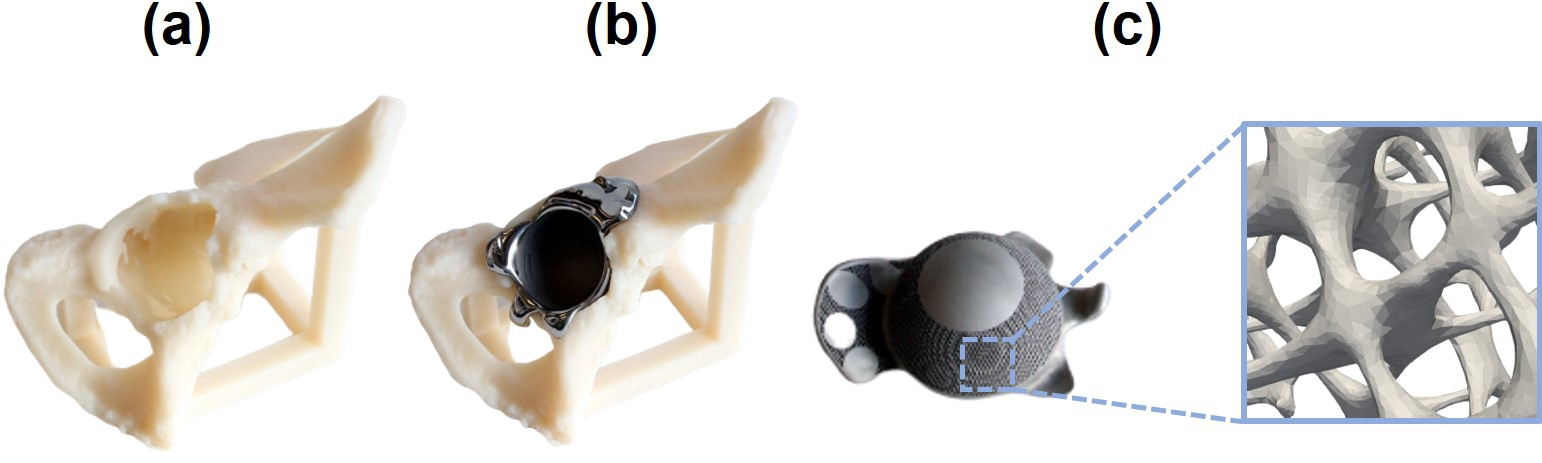
\includegraphics[width=\textwidth]{implant.jpg}
\caption[Application of the acetabular implant]{Demonstration of the application of a porous acetabular implant.} \label{fig:cup_implant}
\end{figure}

\section{Materials and Methods}

\subsection{Topology optimization model}

For building the lattice structure, the in-house developed open-source tool ASLI \cite{Perez-Boerema2022} was used to create a triply periodic minimal surface based infill for the acetabular implant based on the output of a patient-specific topology optimization.

\subsection{Biodegradation model}




In this study, we developed a quantitative mathematical model to predict the biodegradation of magnesium-based implants. Magnesium (Mg) has been selected to start with due to its acceptable mechanical properties, biocompatibility, and contribution in osteoinductivity \cite{Agarwal2016}. The developed model captures the release of Mg ions, the formation of a protective film,  the dissolution of this film due to the presence of various ions in the surrounding environment, and change of pH. This was accomplished by deriving a system of nonlinear time-dependent reaction-diffusion partial differential equations (PDEs) from the underlying oxidation-reduction reactions occurring during the biodegradation process of metallic materials in simulated body fluid. The level-set formalism was employed to track the movement of the biodegradation front between the implant and its surroundings. The equations were solved implicitly using the finite element method for spatial terms (with a 1st order Lagrange polynomial as the shape function) and backward-Euler finite difference method for temporal terms on an Eulerian mesh, implemented in the open-source PDE solver FreeFEM\cite{Hecht2012}. The details of this model can be found in our previous contribution \cite{Barzegari2021}. 

In order to build the computational model, the resulting surface mesh of the topology optimization routine, consisting of \num{5347924} faces, was converted to a volume mesh and embedded in a cubic container that was to act as the environment during the biodegradation simulations. The conversion of the surface mesh was done using GMSH \cite{Geuzaine2009}, and the embedding process was carried out using the internal mesh engine of FreeFEM, called BAMG. The mesh was refined on the implant-environment interface to increase the numerical accuracy of the interface tracking model, leading to a final mesh with \num{45870053} elements. The mesh refinement process was handled using Mmg \cite{Dapogny2014} (and ParMmg \cite{balarac:hal-03344779}). Fig. \ref{fig:cup_model} shows the embedded cup model and a cross section of the final generated mesh, which was refined on the metal-solution interface.



\begin{figure}[h]
\centering
\medskip
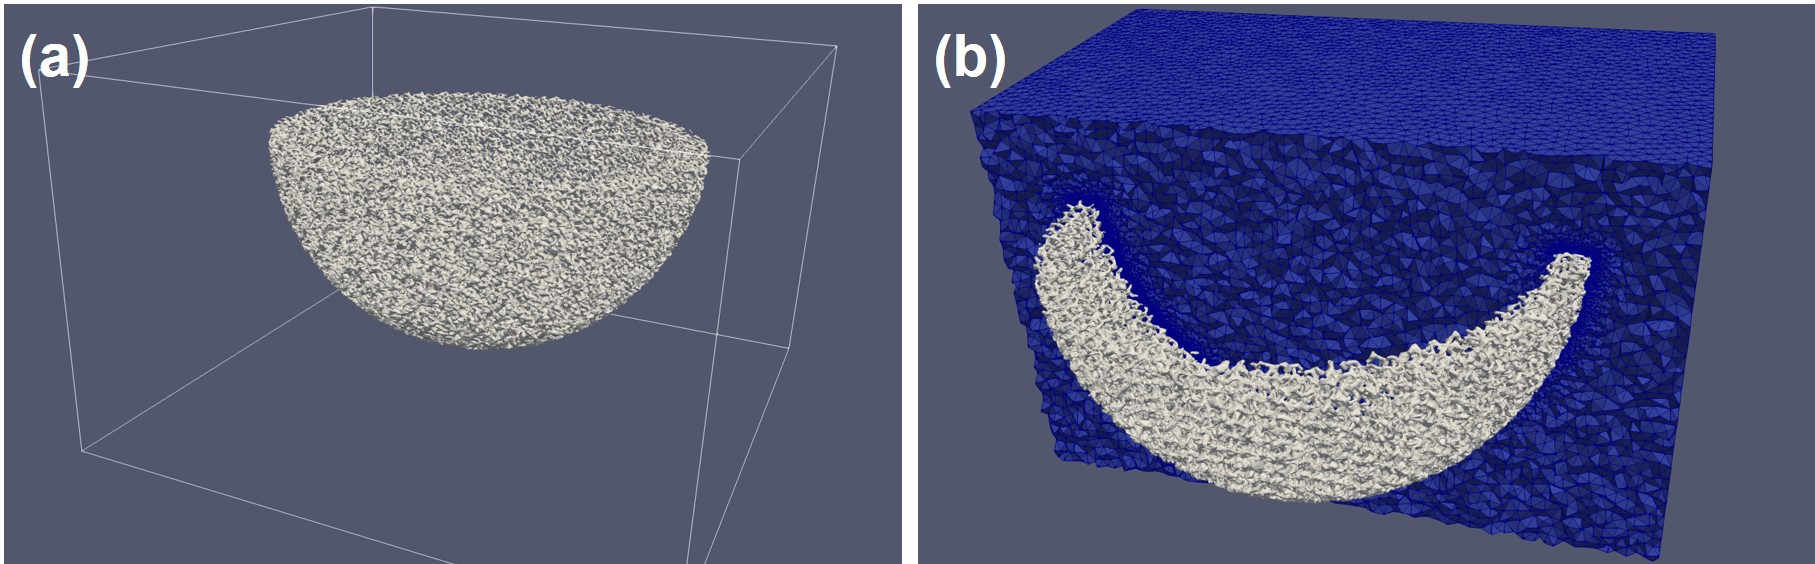
\includegraphics[width=\textwidth]{model.jpg}
\caption[Computational biodegradation model for the porous acetabular implant]{a) The computational biodegradation model for the porous acetabular implant: a)the optimized acetabular implant embedded inside a cubic container, b) a cross section of the generated mesh with the surface of the implant visualized as the light gray surface.} \label{fig:cup_model}
\end{figure}

For dealing with a problem of this size and making the model capable of being scaled in large-scale computing systems, the model was implemented making use of the high-performance computing (HPC) techniques available in the FreeFEM language v4.10 and PETSc toolkit v3.16.1 \cite{petsc}. In this implementation, METIS and ParMETIS graph partitioners \cite{METIS1998} were used to decompose the mesh into various partitions, and then the partitioned mesh was distributed among available computing resources using the HPDDM preconditioner \cite{Jolivet2013}. Fig. \ref{fig:cup_decomposition} shows the decomposition of the computational mesh. Moreover, HYPRE BoomerAMG \cite{Falgout2002} preconditioner and GMRES iterative solver \cite{Saad1986} were used to solve the linear systems of equations obtained from applying the finite element discretization on the model. More details of the implementation can be found in \cite{Barzegari2022}.

\begin{figure}[h]
\centering
\medskip
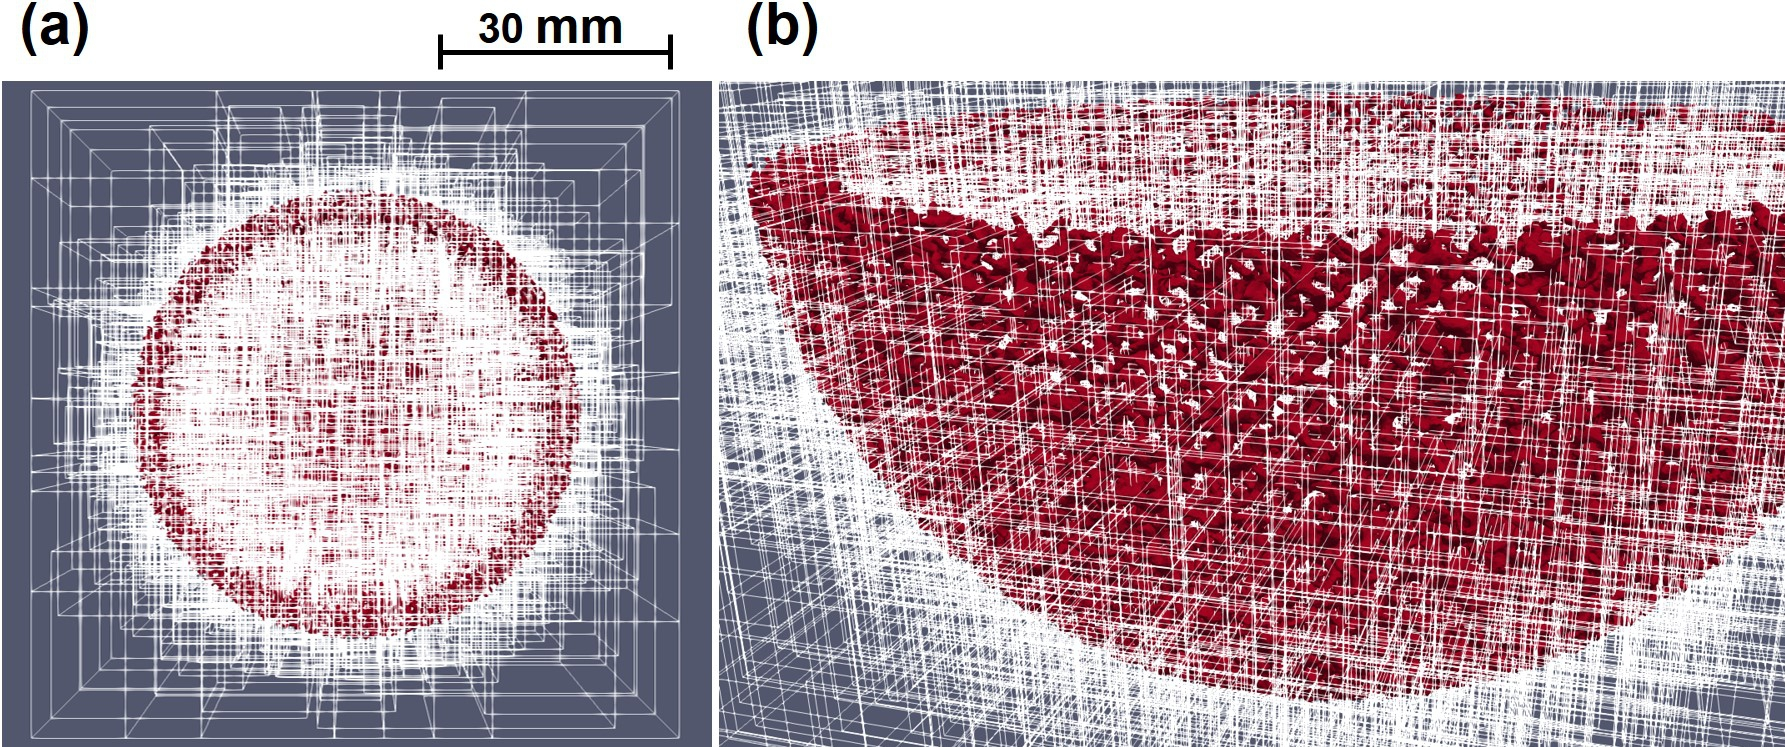
\includegraphics[width=\textwidth]{decomposition.jpg}
\caption[Mesh decomposition of the acetabular implant model]{Mesh decomposition of the computational biodegradation model to be distributed to available computing nodes, a) top view, b) perspective side view. } \label{fig:cup_decomposition}
\end{figure}

The simulation was carried out using 2,000 CPU cores with 16.5 TB of available memory on Dutch national supercomputer, Snellius. The simulation results, comprising of \num{95000} files with a total size of 148 GB, were visualized using a parallel client-server remote rendering approach in ParaView server v5.9.1 running on 128 CPU cores on the ARCHER2 supercomputer. 

In order to obtain the scaling behavior of the model in an HPC environment, strong and weak scaling tests were performed in the Snellius supercomputer. For the weak scaling test, in addition to the mesh with \num{45870053} elements, two more mesh files consisting of less elements were generated using the aforementioned procedure for embedding and refining the mesh. These models had \num{15989521} and \num{29035491}, respectively, to which the number of employed CPU cores were adjusted accordingly. The strong scaling test was carried out for all the three model sizes by varying the number of employed CPU cores from 60 to \num{9000}. 


\section{Results and Discussion}

The generated lattice structure of the implant, infilled by skeletal-gyroid unit cell type, is depicted in Fig. 1A. Biodegradation results show that the acetabular implant degrades faster in the region with higher porosity, i.e. the region with more exposed surface area to the environment (Fig. 1B). Loss of material over time was found to be in line with the values obtained in our previous study \cite{Barzegari2021}, showing that scaling the model in an HPC environment does not affect the quantitative predictions made by the model.  The scaling tests show that the optimal size for the distributed computing environment is \num{5000} CPU cores, above which no significant improvement in the execution time was observed.

\begin{figure}[h]
\centering
\medskip
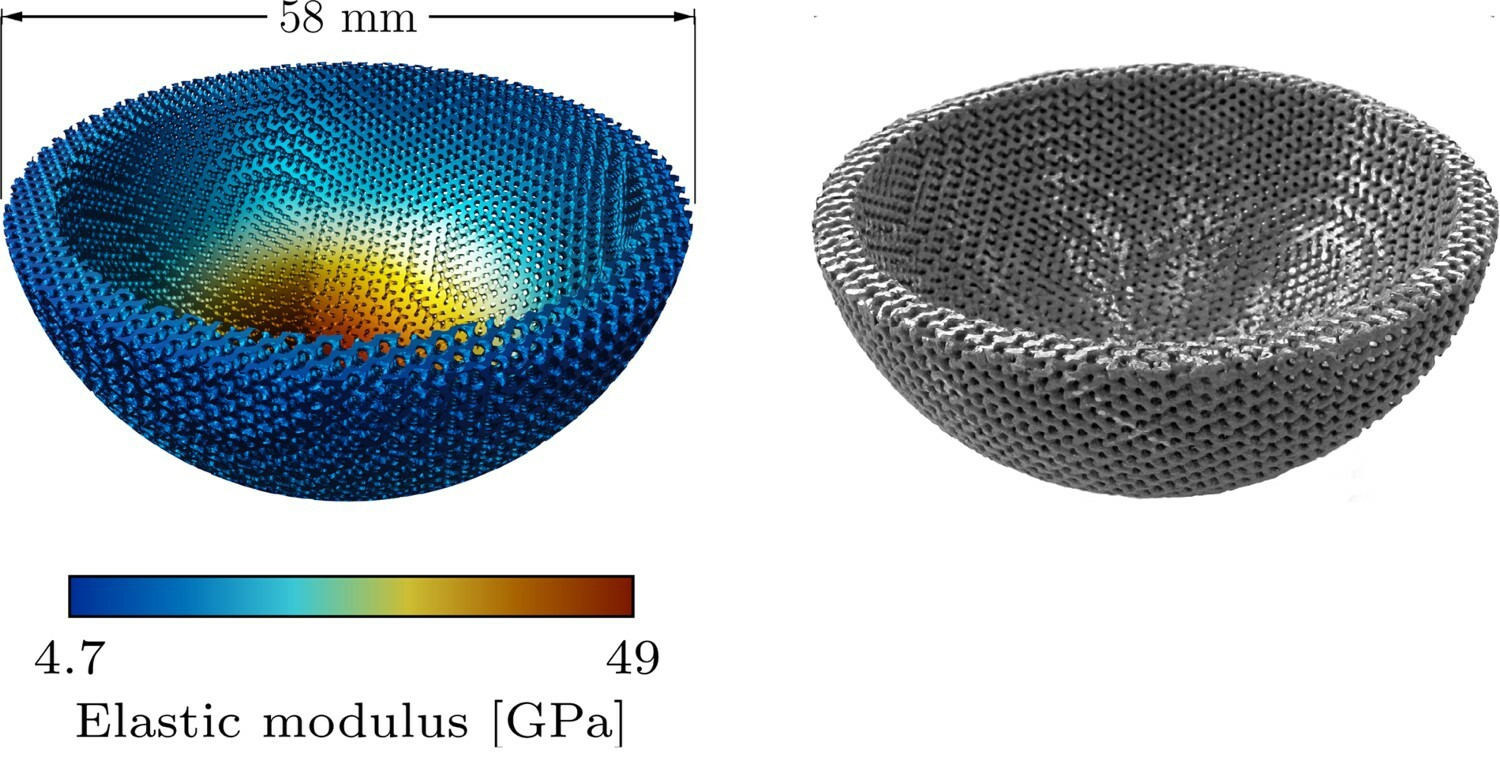
\includegraphics[width=\textwidth]{optimization.jpg}
\caption[Infilled acetabular implant]{Acetabular implant infilled by varying volume fraction to match a desired stiffness distribution.} \label{fig:cup_optimization}
\end{figure}

\begin{figure}[h]
\centering
\medskip
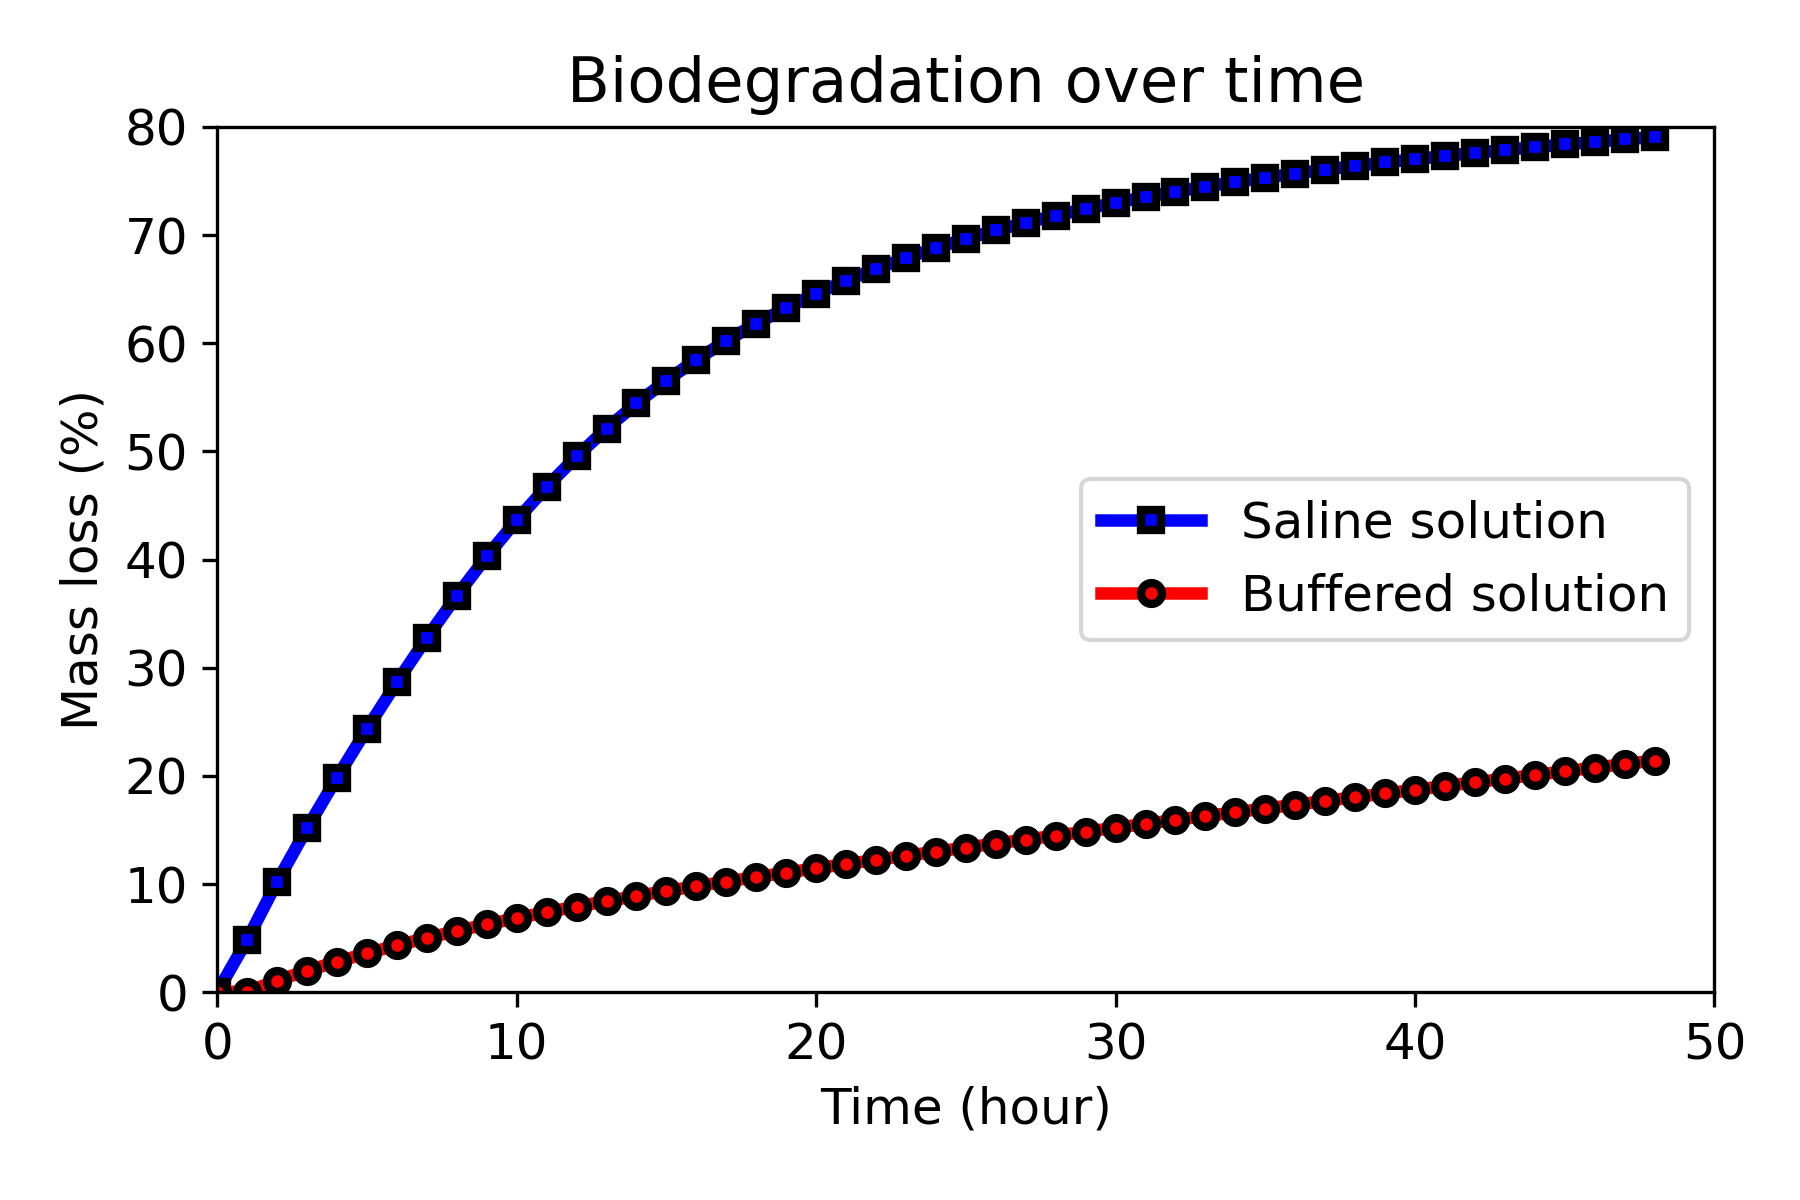
\includegraphics[width=0.9\textwidth]{degradation_rate.png}
\caption[Biodegradation rate for the acetabular implant]{Rate of mass loss during the biodegradation of the porous acetabular implant in saline and buffered solutions.} \label{fig:cup_degradation_rate}
\end{figure}

\begin{figure}[h]
\centering
\medskip
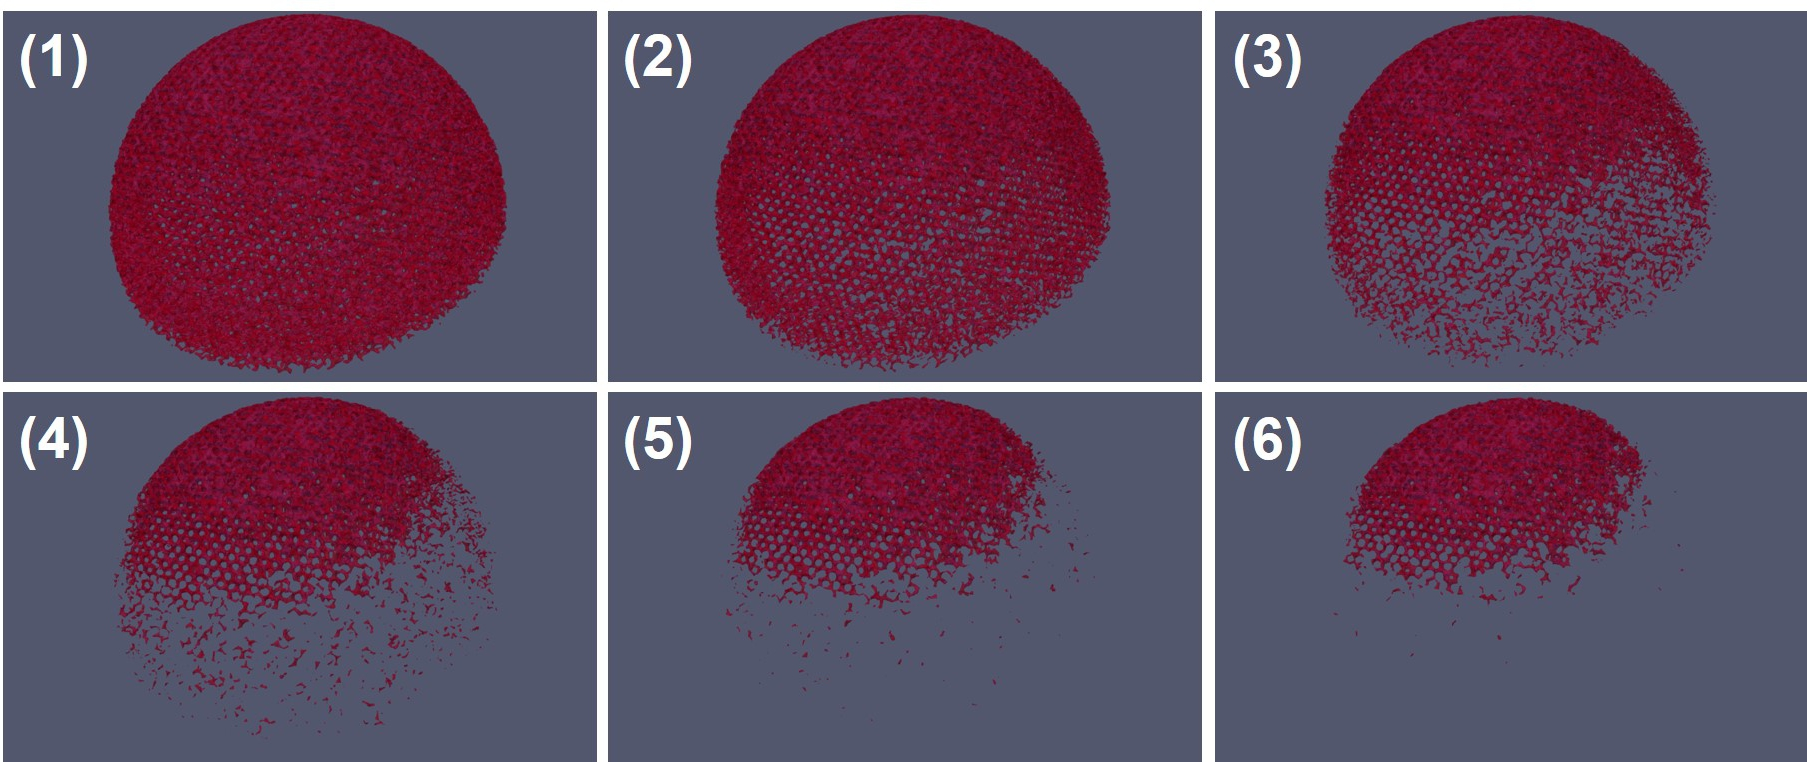
\includegraphics[width=\textwidth]{degradation_visual.jpg}
\caption[Visualization of the change of morphology of the acetabular implant]{Visualization of the change of morphology of the acetabular implant.} \label{fig:cup_degradation_visual}
\end{figure}

\begin{figure}[h]
\centering
\medskip
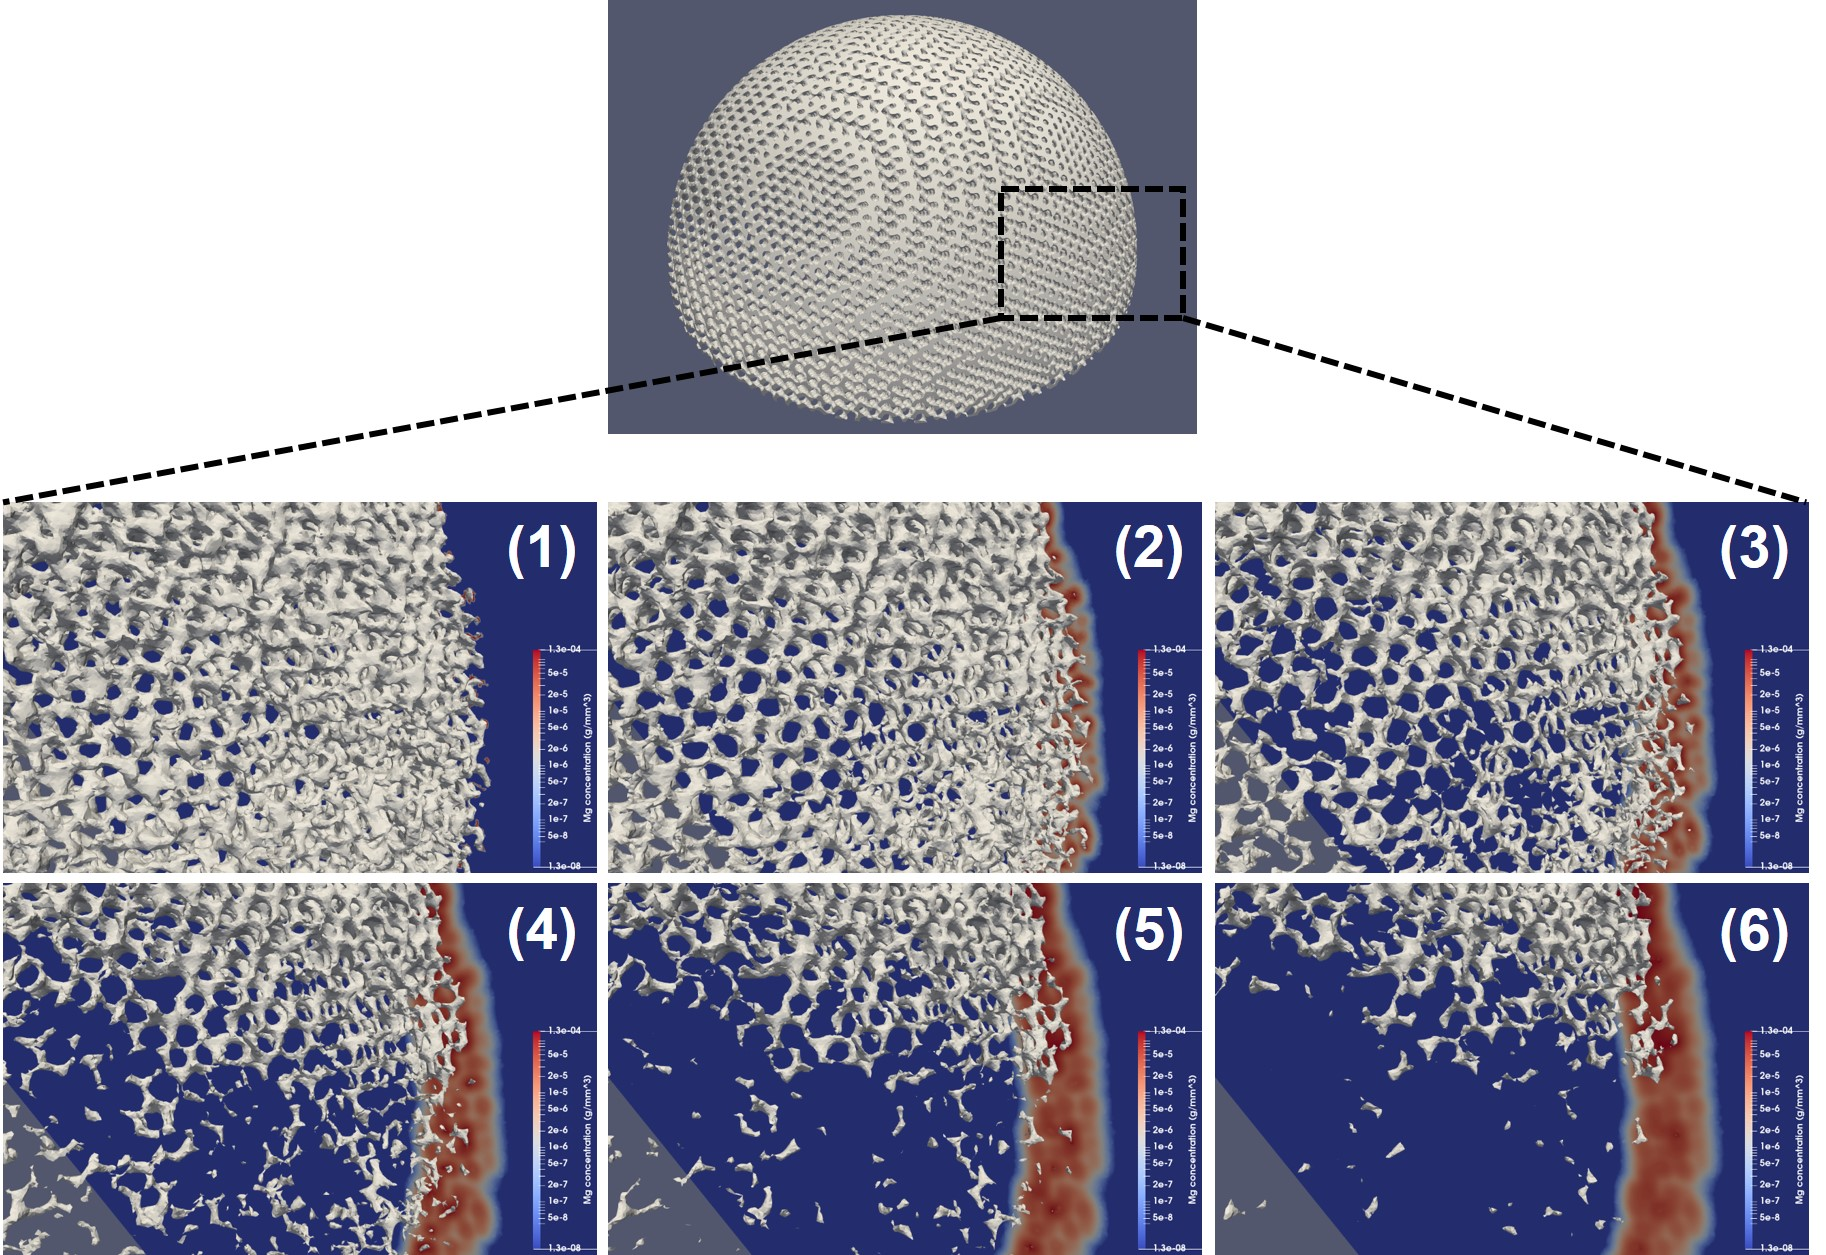
\includegraphics[width=\textwidth]{degradation_visual_close.jpg}
\caption[Visualization of the change of morphology of the acetabular implant]{Visualization of the change of morphology of the acetabular implant - zoom view.} \label{fig:cup_degradation_visual_close}
\end{figure}

\begin{figure}[h]
\centering
\medskip
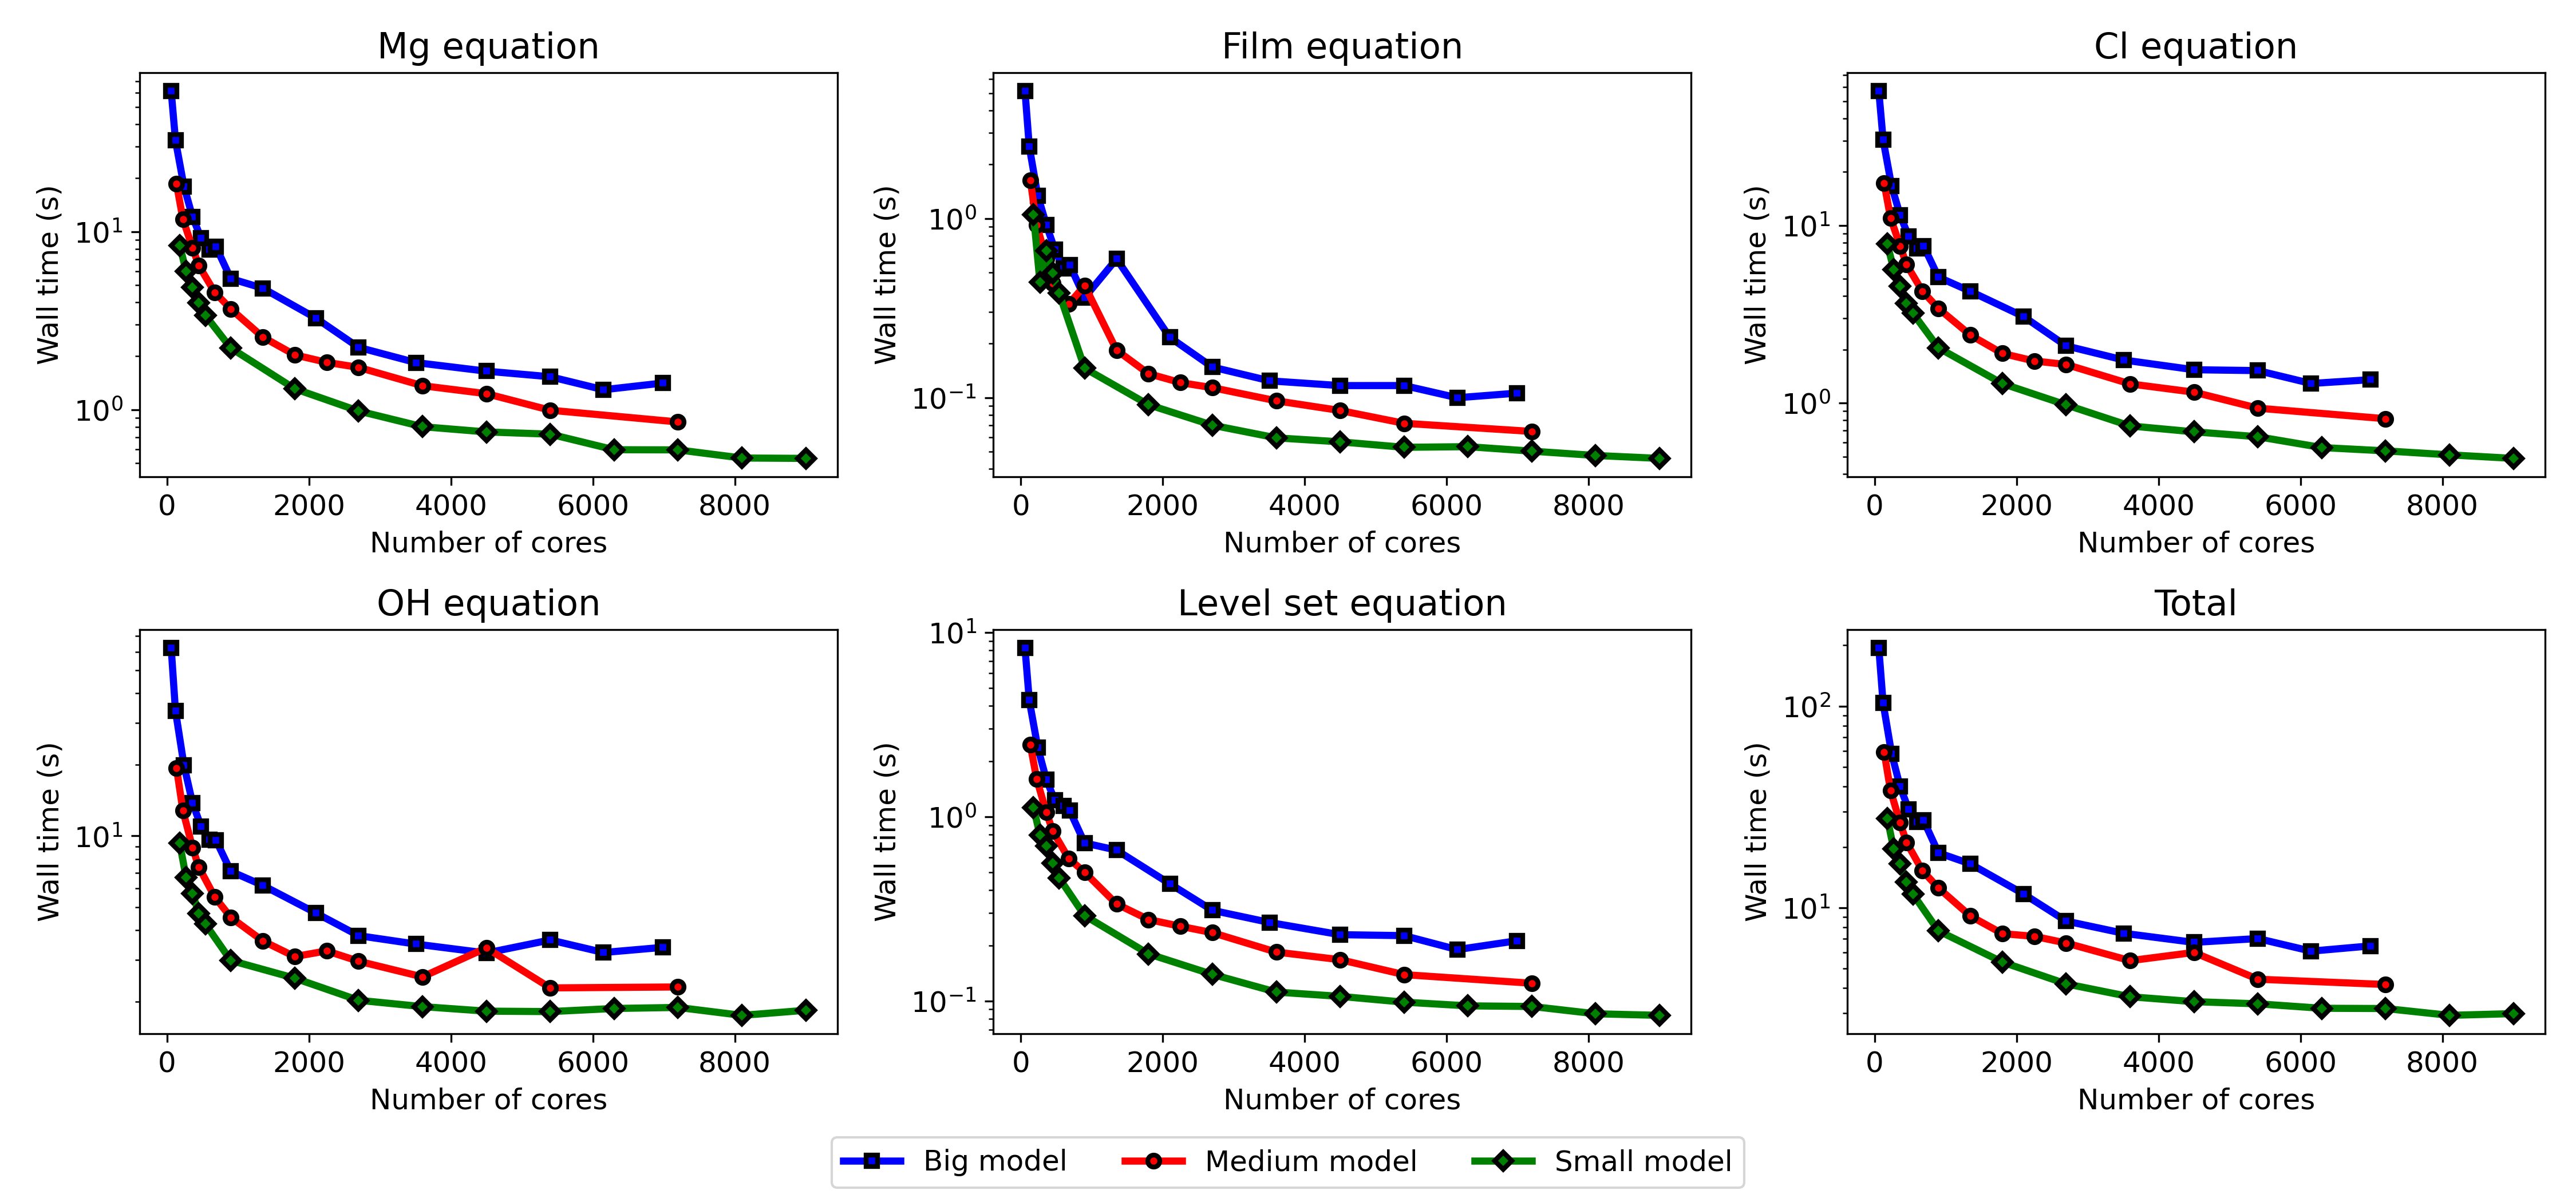
\includegraphics[width=\textwidth]{strong_scaling.png}
\caption[Strong scaling of individual components of the biodegradation model]{Strong scaling of individual components of the biodegradation model.} \label{fig:cup_strong_scaling}
\end{figure}


\begin{figure}[h]
\centering
\medskip
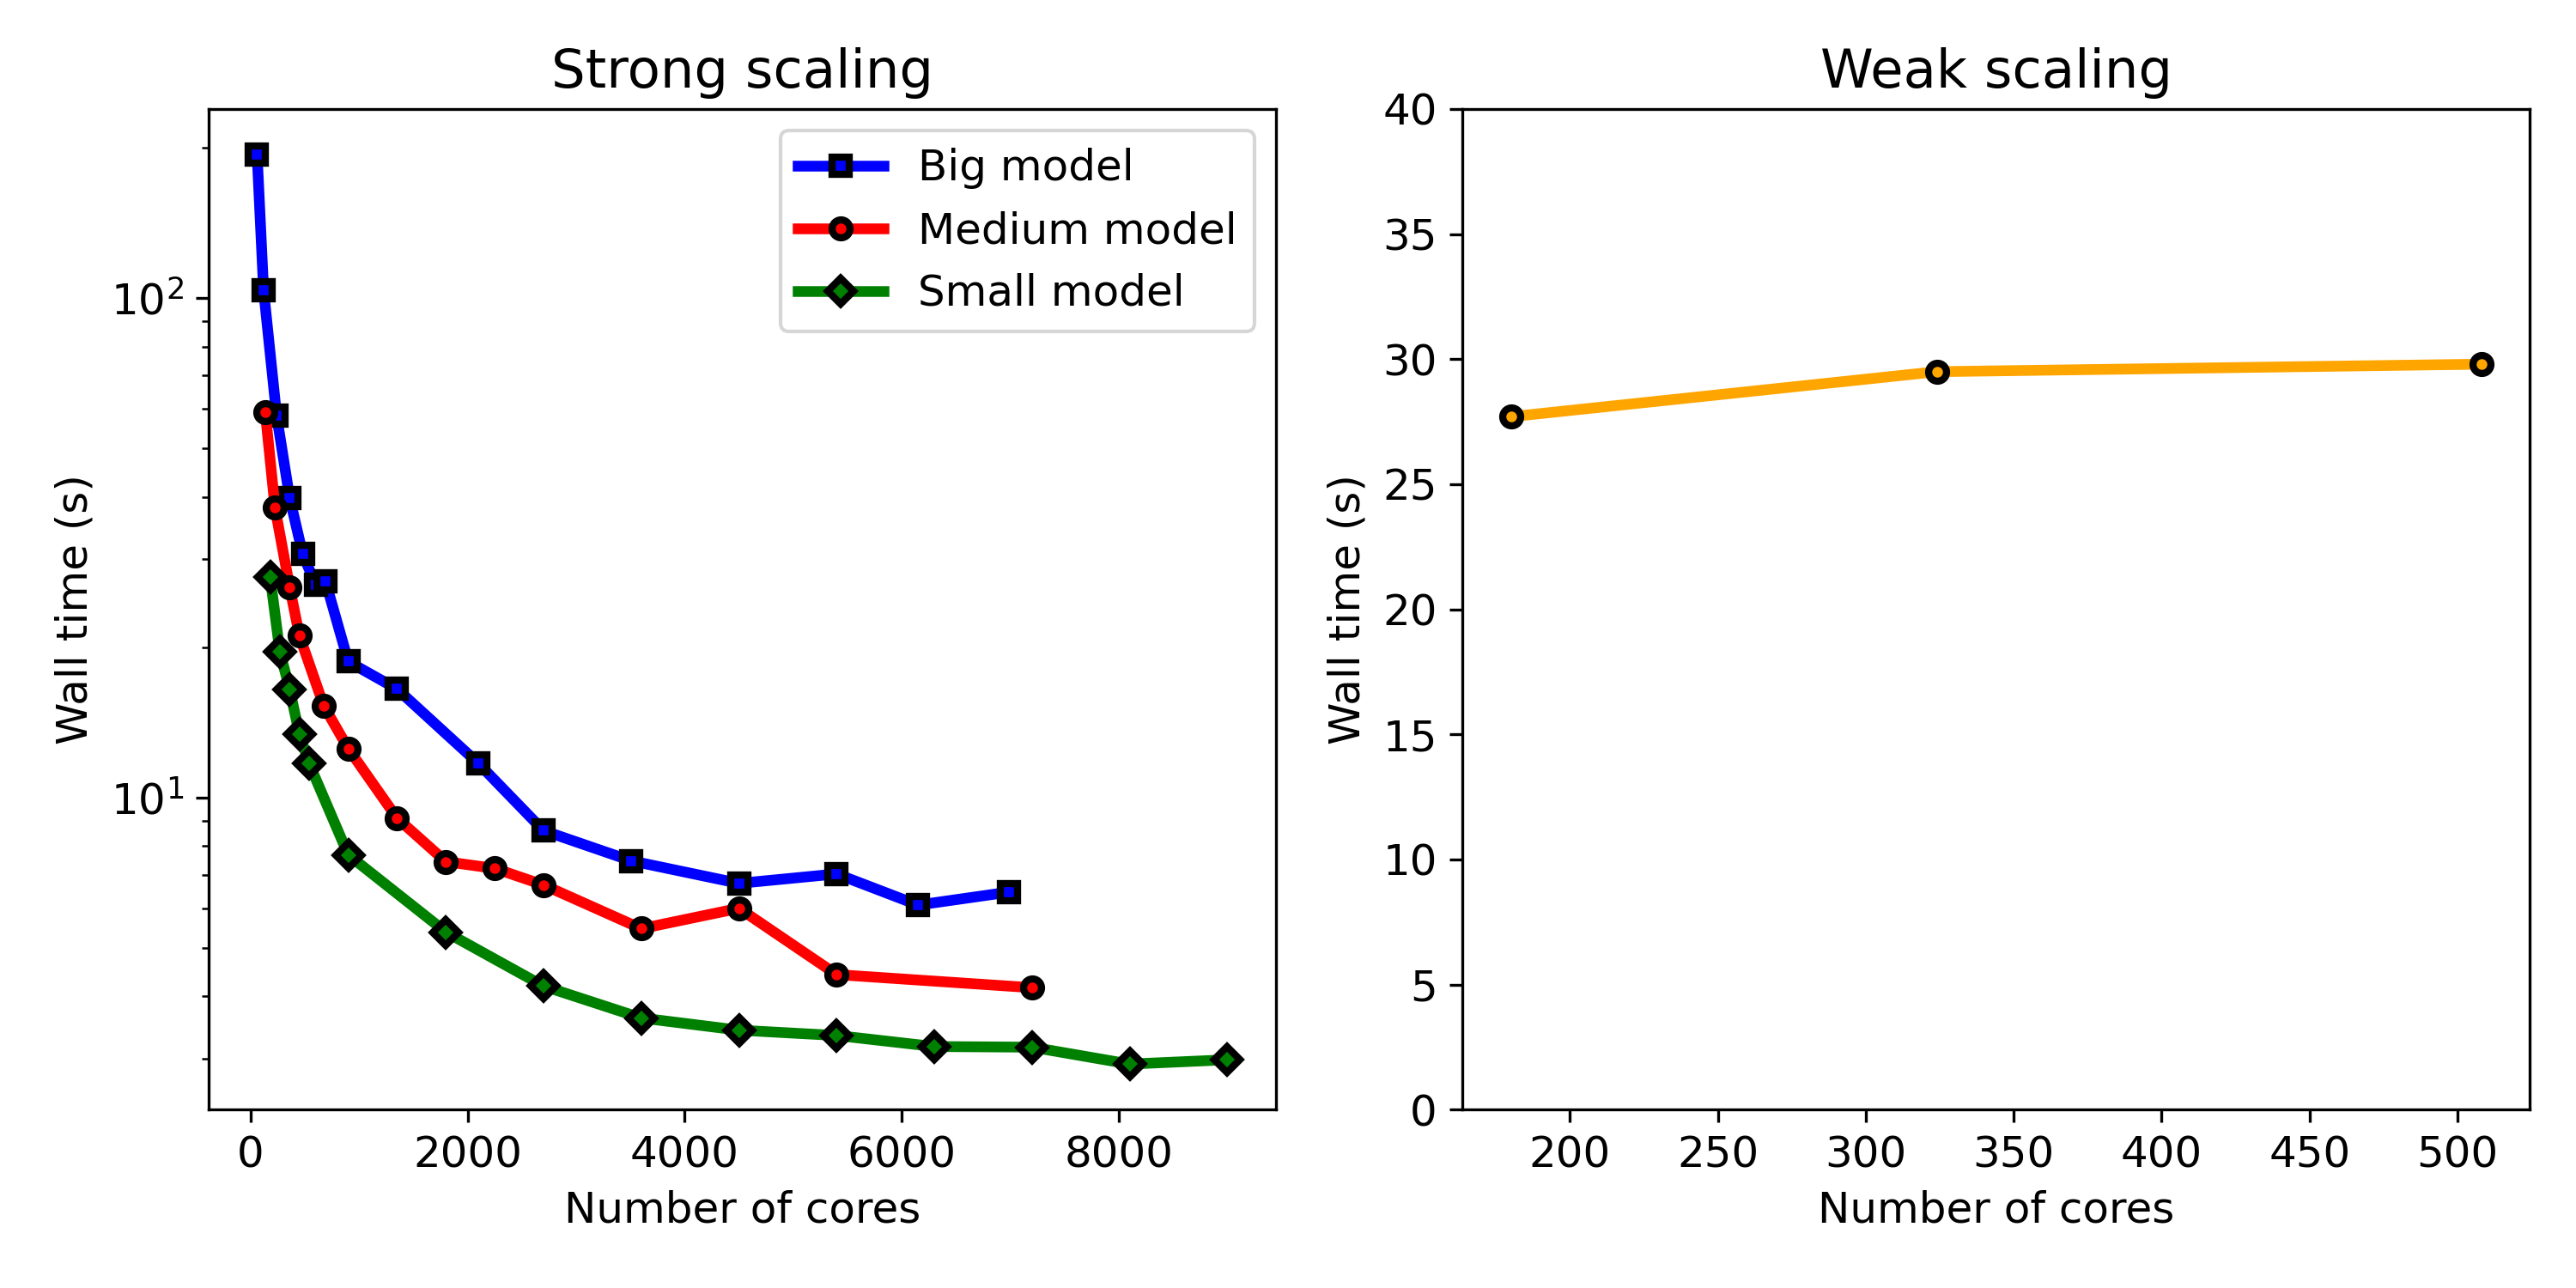
\includegraphics[width=\textwidth]{weak_strong.png}
\caption[Weak and strong scaling of of the acetabular implant model]{Weak and strong scaling of of the computational biodegradation model of the acetabular implant.} \label{fig:cup_weak_strong}
\end{figure}

\section{Conclusions}

In this work, taking advantage of HPC techniques to simulate a large-scale 3D model led to a computational model capable of predicting the biodegradation behavior of an acetabular implant in high resolution. Results demonstrate the potential of the model to act as a tool for assessing and tuning the biodegradation properties of orthopedic  implants regardless of shape or complexity.

\section{Acknowledgments}

Funded by Interreg VA Flanders - Netherlands, (2014TC16RFCB046, Prosperos) \& FWO-Vlaanderen (G085018N).

Dutch supercomputer - Snellius

UK supercomputer - ARCHER2


\begin{subappendices}

\section{Challenges in scaling the computational model to thousands of CPU cores}

%Building with different MPI implementations
%Inter-node communication
%Running parallel FF
%Mesh generation (parallel, sequential)
%Converting surface mesh to volume
%Scaling issues
%Memory issues
%Node types
%Visualization, GPU nodes
%Partitioning (METIS, ParMETIS)
%Storage
%Solving NS equation

\end{subappendices}


%%%%%%%%%%%%%%%%%%%%%%%%%%%%%%%%%%%%%%%%%%%%%%%%%%
% Keep the following \cleardoublepage at the end of this file, 
% otherwise \includeonly includes empty pages.
\cleardoublepage

